% ========================================
% CHAPTER 4: METHODS (CONCEPTUAL: ARCHITECTURE, DATA, AND TRAINING PROCEDURES)
% ========================================
\chapter{Methods}

\textbf{note: here I write "what am i doing on top of other methods" I write it conceptually. if i need results maybe reference to the next chapter.}



% ========================================
% SECTION 4.1: CONCEPTUAL SETUP AND AGENTIC DATA ACQUISITION
% ========================================
\section{Data Acquisition and Setup}

\subsection{SWE-bench}
We have chosen to use the SWE-bench \cite{jimenez2024swebench} dataset for our experiments.
It is a well known dataset for evaluating the performance of SWE agents.
It contains a large number of SWE tasks, each with a set of instructions and a set of expected outputs.
They were collected from real life GitHub issues. 
We have chosen to work with a subset -- SWE-bench Verified \cite{swebench-verified}.
It is a subset of the SWE-bench dataset that contains only the tasks that have been verified to be correct.

\subsection{Tools and Interaction Protocol (setup?)}
We follow the SWE-smith setup for SWE-bench Verified \cite{jimenez2024swebench}, where the assistant agent interacts with the environment through a minimal toolset and a fixed protocol. 
Concretely, the available tools are a shell interface (\texttt{bash}), a submission tool (\texttt{submit}), and a custom editing utility (\texttt{str\_replace\_editor}).
These tools generate the observations that accumulate within the trajectory context.
The exact SWE-smith prompt (and the tools description) is provided in Appendix~\ref{app:swe-smith-prompt}.
It should be noted that this method does not use function calling functionality of the model. 
While some models support a special format for function calling (e.g. additional fields for the tools descriptions etc.), in this case we just use the tools as described in the prompt.

\paragraph{The \texttt{str\_replace\_editor}.}
This is a stateful file editor that supports viewing, creating, and editing files with precise, line-exact operations.
Its state persists across steps, enabling consistent multi-edit workflows. 
The interface exposes the following commands: \texttt{view}, \texttt{create}, \texttt{str\_replace}, \texttt{insert}, and \texttt{undo\_edit}. 

For deterministic edits, \texttt{str\_replace} requires \texttt{old\_str} to match exactly one or more consecutive lines in the target file, including whitespace.
The \texttt{new\_str} content replaces the matched block.
The \texttt{insert} command appends \texttt{new\_str} after a specified line number.

By this, there is a lot of tools combined into one, but it works well as described in \cite{swe-smith}, so we adopt it. 
And also to be comparable to other open sourced scores.

\subsection{Agentic Trajectories as Data}
We treat sequential action--observation interactions (trajectories) as training data.
These trajectories were obtained using a strong teacher model (e.g., Claude Sonnet 3.7) on the SWE-bench Verified dataset to produce high-quality inputs suitable for futher training.
The setup for generating these trajectories follows the SWE-smith setup closely\cite{swe-smith}.

% ========================================
% SECTION 4.2: ICAE MODEL ARCHITECTURE FOR AGENTIC APPLICATION
% ========================================
\section{ICAE Model in Agentic Setup}

\subsection{ICAE Components}
As described previously, the ICAE \cite{ge_context_2024} consists of two modules: a lightweight encoder (implemented via a LoRA-adapted LLM) and a fixed decoder (the LLM itself).
The encoder processes the long trajectory context and generates a fixed number of learnable memory token.

We use the encoder for every environment observation (\textbf{TODO: picture here?})
So, more in detail, the encoder is only applied if all of the next are true:
\begin{itemize}
  \item The text is an observation (i.e. response from the environment, not the action)
  \item The text is longer or equal than 256 tokens
\end{itemize}
The actions are short and do not require compression, while the observations can be long and complex.
Due to the nature of the ICAE framework, the compression produces a fixed number of memory tokens, which we fix at 256.
Applying the encoder to the shorter texts would be a waste of resources and would create a mismatch between the training and the validation settings.
You can see the example of this in figure \ref{fig:ser1} and \ref{fig:ser2} from Chapter~\ref{chap:5}.

The ICAE framework design turns a long, potentially unwieldy context into a compact representation that the decoder can efficiently consume, improving latency and memory footprint while preserving fidelity for downstream tasks. 
The number of memory tokens controls the compression ratio (e.g., $4\times$ or higher), and the position-ID placement of these tokens influences how readily the decoder can access stored information (cf. Section~2.1) \cite{ge_-context_2024}.

Beyond the high-level description, Figure~\ref{fig:icae} depicts the encoder–decoder split. 
On the left, the encoder ingests the full context (e.g., a text) and produces a fixed number of memory tokens. 
On the right, the frozen decoder receives these tokens and a tokens
During pretraining, the encoder is optimized so that the decoder can reconstruct the original text and continue language modeling (50/50 chance of being used).
During fine-tuning, the objective emphasizes answering prompts correctly given only the memory tokens and the task prompt.
In practice, the encoder is frequently adapted with parameter-efficient methods such as LoRA \cite{hu2021lora}, whereas the decoder remains frozen to preserve the capabilities of the base model.
\begin{figure}[hbt]
  \centering
  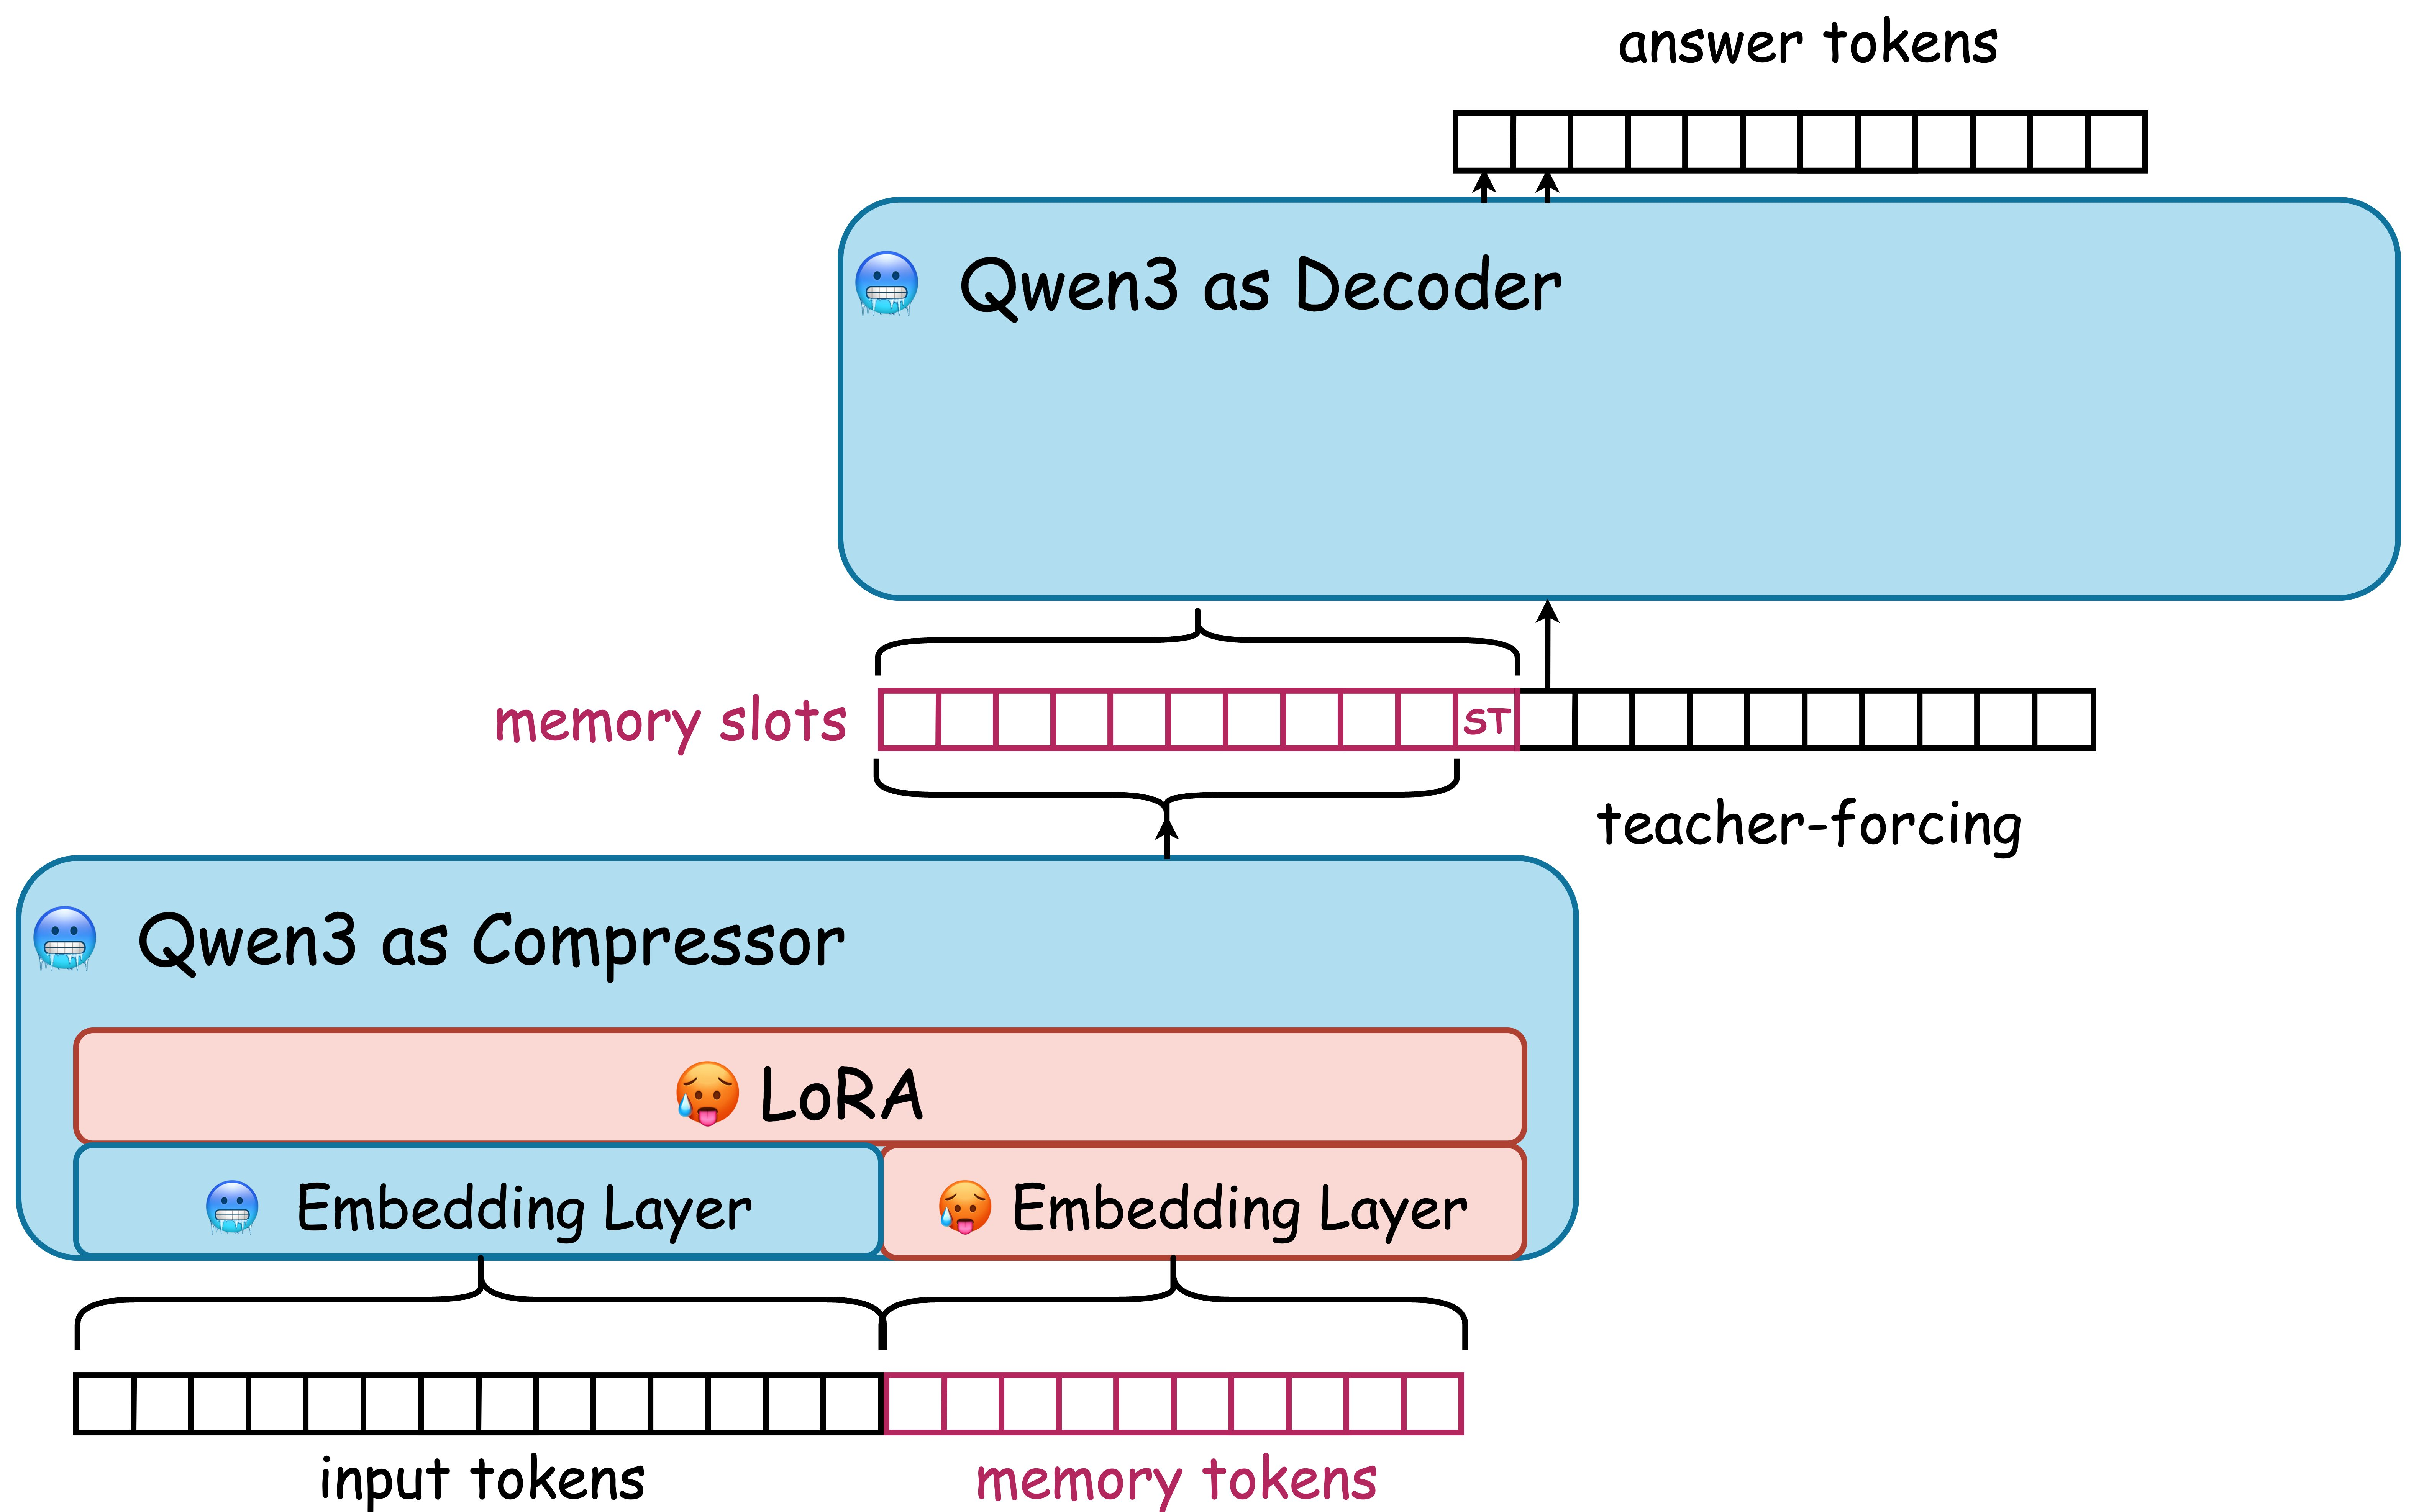
\includegraphics[width=0.8\textwidth]{graphs/icae.jpeg}
  \caption{In-Context Autoencoder (ICAE) framework architecture}
  \label{fig:icae}
\end{figure}

\subsection{Base Model Configuration (Qwen3)}
We use the Qwen3 model family (specificaly Qwen3-8B) as the base LLM. 
To make things simpler, we explicitly disable long-form "thinking" during decoding by inserting the token sequence \texttt{\textbackslash think \textbackslash think} with a newline marker (\texttt{\textbackslash n}) in between.
This is exactly how the authors of \cite{qwen3} recommend disabling thinking.
This prefix makes the model "believe" it has already produced intermediate thoughts (empty in this case), while in fact no additional content is generated.
We found that deleting or leaving this prefix in the history does have an inretesting affect the quality of the model, we describe this in more detail in Section~\ref{sec:5.6}.

It should also be noted that the authors of \cite{ge_context_2024} have only worked with older models (such as Llama2 and Mistral-v0.1), and only publish the weights of the latter.


% ========================================
% SECTION 4.4: TRAINING PROCEDURES BASED ON QWEN3
% ========================================
\section{Training Procedures and Evaluation}

\subsection{Pretraining (PT)}
Our pretraining procedure follows the original ICAE formulation~\cite{ge_-context_2024}.
We use two primary self-supervised objectives:
\begin{enumerate}[label=(\roman*)]
    \item \textbf{Autoencoding (AE)}, where ICAE restores the original input text from its memory slots (prompted by a special token \texttt{[AE]}).
    \item \textbf{Language Modeling (LM)}, which predicts the continuation of the context (prompted without any special tokens) to improve generalization and prevent overfitting to the AE task.
\end{enumerate}
This pretraining was performed on the dataset SlimPajama-6B \cite{pajama6b}\footnote{\url{https://huggingface.co/datasets/DKYoon/SlimPajama-6B}}.
It is a common text dataset, that is used for pretraining LLMs, consisting of 6 billion tokens (a random 1\% of the original 627B tokens).
The dataset that authors used in their original paper "The Pile" was unavailable.

It should be noted that only LoRA weights of the encoder are trained here (specifically only form Q and K matrices of the attention layers).
So, in theory, we are training the encoder to encode the context into such embeddings, that the decoder will be able to reconstruct the original context from them or to continue the text from the context.

\begin{figure}[hbt]
  \centering
  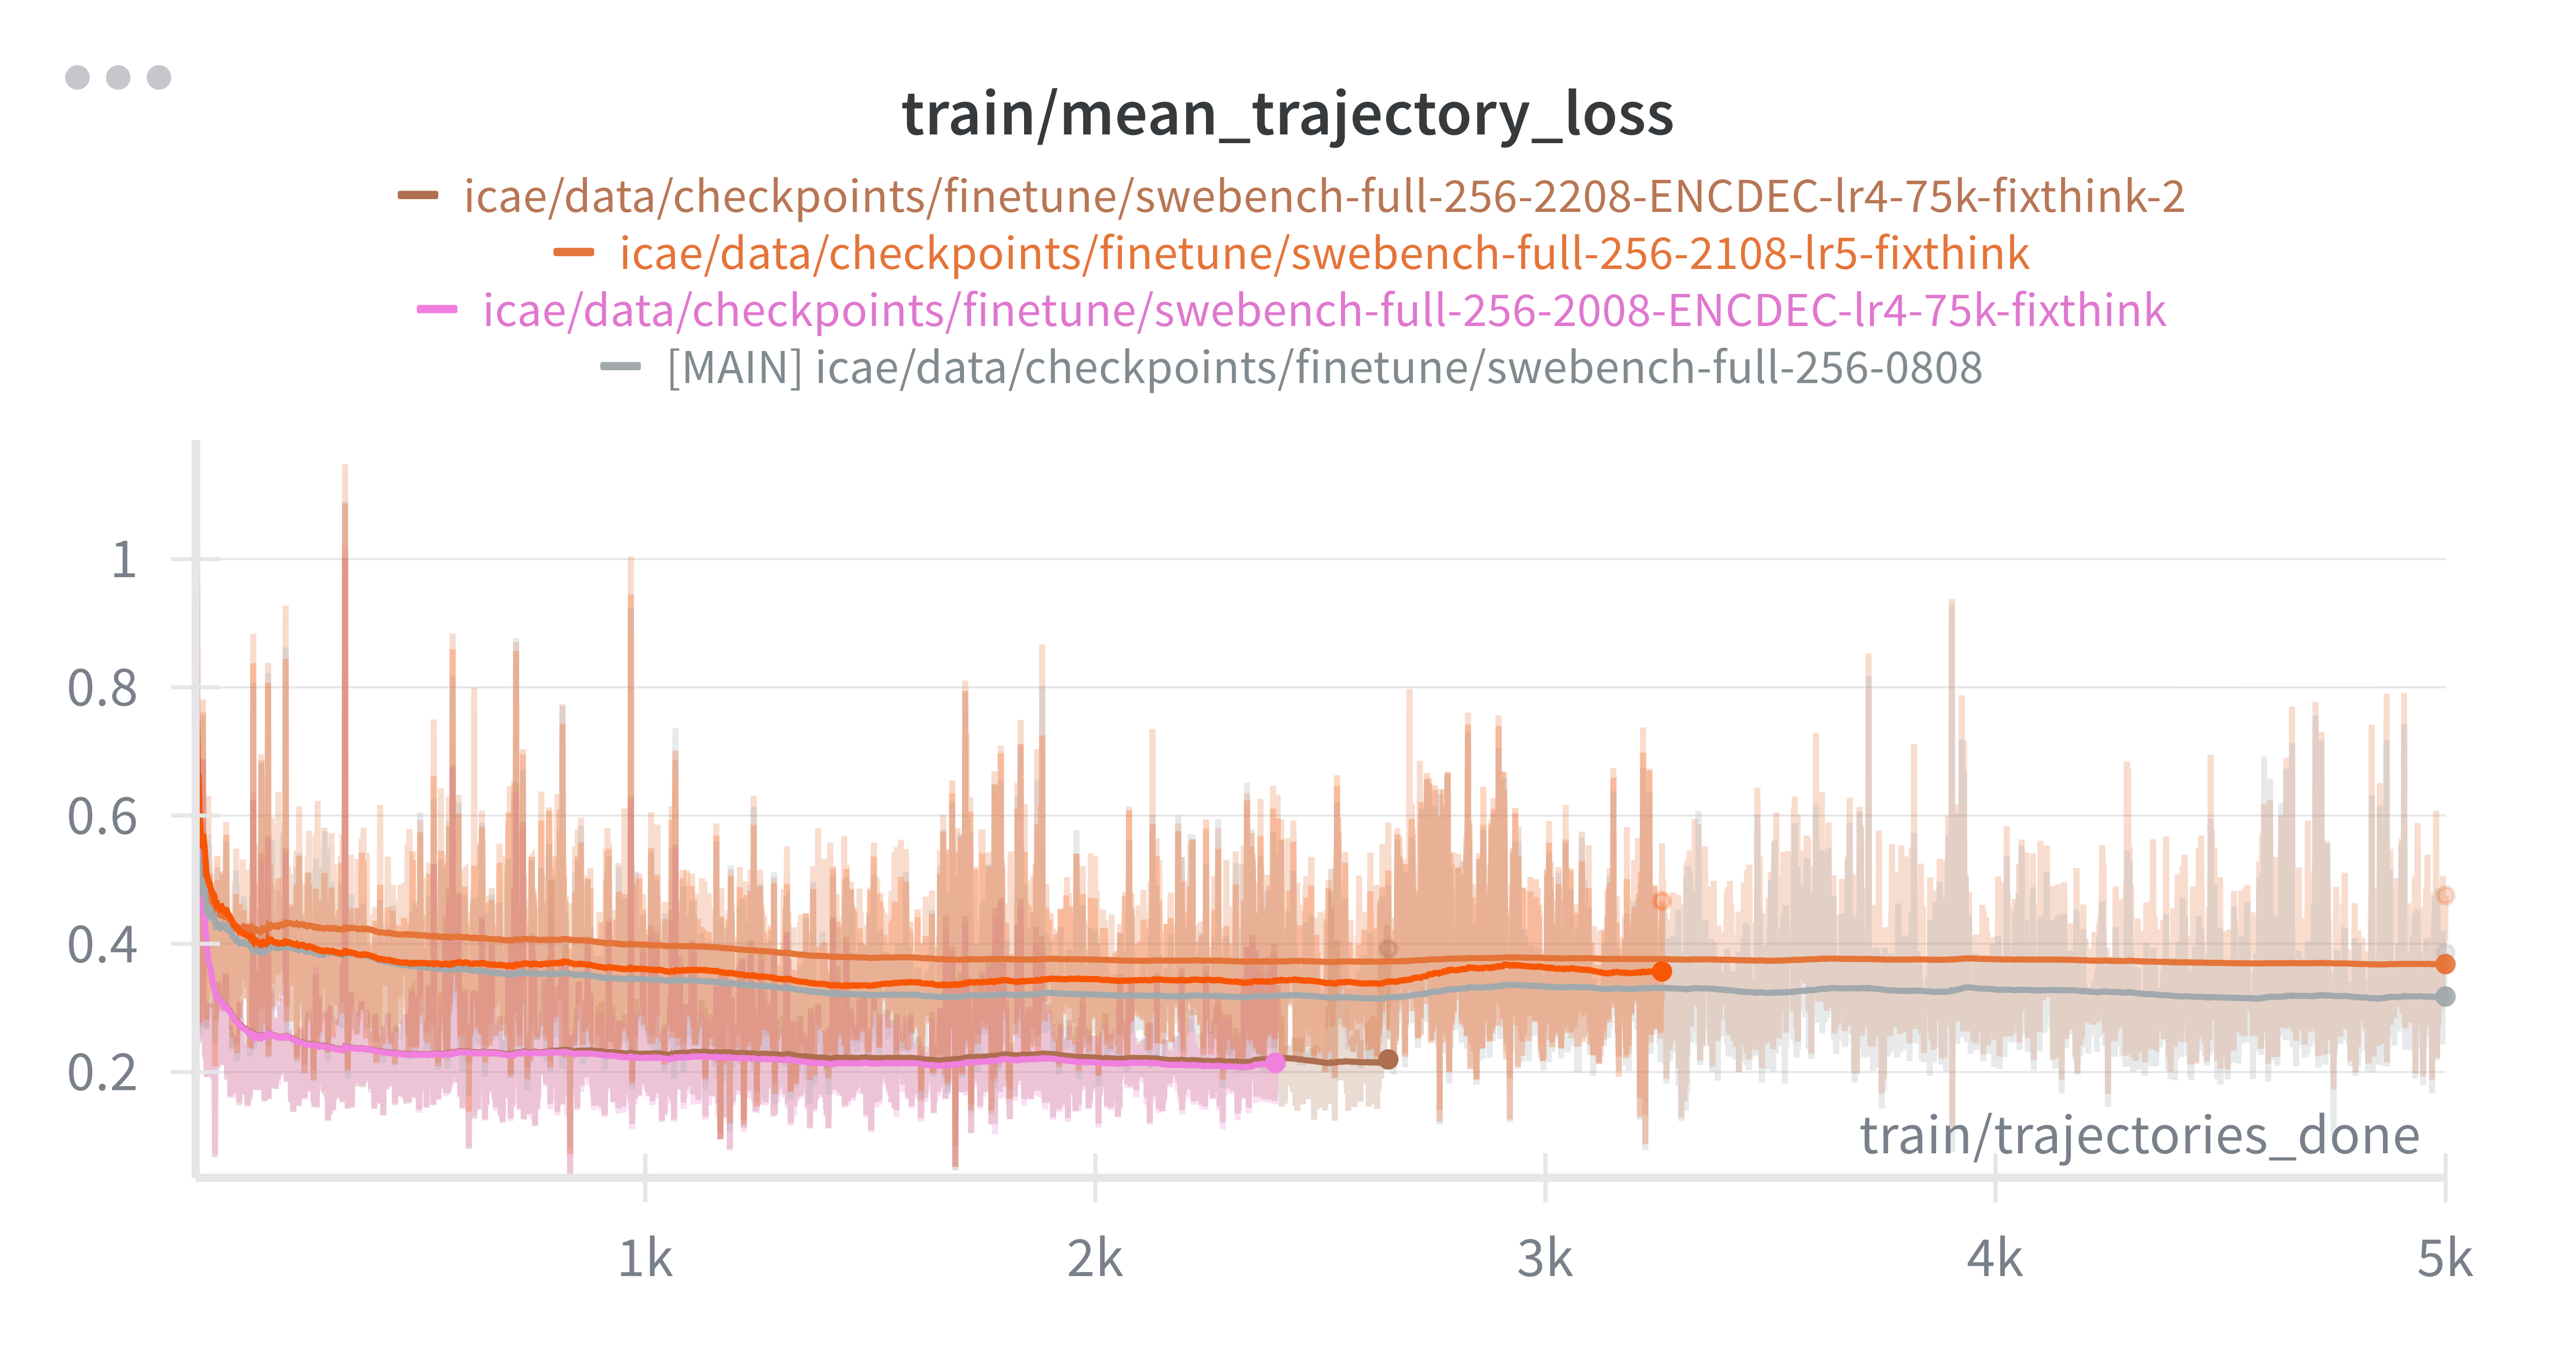
\includegraphics[width=0.9\textwidth]{graphs/pt_losses.png}
  \caption{Pretraining loss curves averaged by trajectory}
  \label{fig:pt_losses}
\end{figure}

\subsection{Fine-Tuning (FT)}
After pretraining, ICAE is fine-tuned using trajectories from SWE-bench Verified (the proccess of obtaining trajectories is described in Section~4.1.3).
Here as well only the LoRA weights are trained.
The fine-tuning objective maximizes the probability of generating the correct agent action (i.e. tool call) conditioned on the memory slots (if the encoder is applied at the current step) and the previous history (???)

It should be noted that the training is only applied to the encoder part, while the decoder is frozen.


During training, the backpropagation process constrains us to optimize over single-step transitions:
So at timestep \(k\), the encoder compresses the observation \(o_{k-1}\) into embeddings. Then, the decoder generates the action \(a_k\) given the memory slots and the previous history.
Then, token-by-token of \(a_k\) we backpropagate the loss through the decoder and the encoder, making an update of the LoRA weights of the encoder.
Crucially, whenever an observation exceeds 256 tokens, the encoder compresses it into a fixed set of 256 memory tokens (continuous embeddings), and these memory tokens replace the original text in the accumulated history.
If the observation is longer than 1024 tokens, we apply the encoder multiple times, preserving the compression ratio, following the authors of \cite{ge_context_2024}.
Consequently, the model never processes the full raw text of long observations during subsequent steps—it only conditions on the compact memory representations.

For example, consider a trajectory:
\begin{enumerate}
  \item \textbf{System prompt} (text): initial instructions and tool descriptions.
  \item \textbf{Task description} (text): user-provided issue or goal.
  \item \textbf{Action 1} (text): e.g., \texttt{bash: ls -la}.
  \item \textbf{Observation 1} (short text, $<256$ tokens): directory listing, kept as-is.
  \item \textbf{Action 2} (text): e.g., \texttt{str\_replace\_editor: view file.py}.
  \item \textbf{Observation 2} (long text, $\geq 256$ tokens): entire file content, compressed into 256 memory tokens.
  \item \textbf{Action 3} (text): e.g., \texttt{str\_replace\_editor: str\_replace ...}.
  \item \textbf{Observation 3} (long text): edit confirmation with context, again compressed into memory tokens.
  \item \textbf{Action 4} (text): e.g., \texttt{bash: pytest}.
  \item \textbf{Observation 4} (short text): test results summary, kept as text.
  \item \textbf{Action 5} (text): \texttt{submit}.
  \item \textbf{End}.
\end{enumerate}
So, in this example, the encoder is applied 2 times (steps 7 and 9), while the decoder is applied 5 times (steps 3, 5, 7, 9, 11).

At training time, each step's loss is computed independently: the model learns to predict \(a_k\) from the prefix ending at \(o_{k-1}\), where any long observation has already been replaced by its memory tokens.
At inference time, the same replacement occurs dynamically, ensuring consistency between training and deployment.
This design allows the model to handle arbitrarily long trajectories without exceeding context limits, as the effective history remains compact.

On figure \ref{fig:ft_losses} you can notice the sudden drop of the loss.
This is phenomenon found in \cite{PI}.
It appears due to the modification of positional encodings for the memory tokens.
We see the effect being the same as described by the authors.
In our experiments, it only appers if we apply the positional encodings manipulations.

\begin{figure}[hbt]
  \centering
  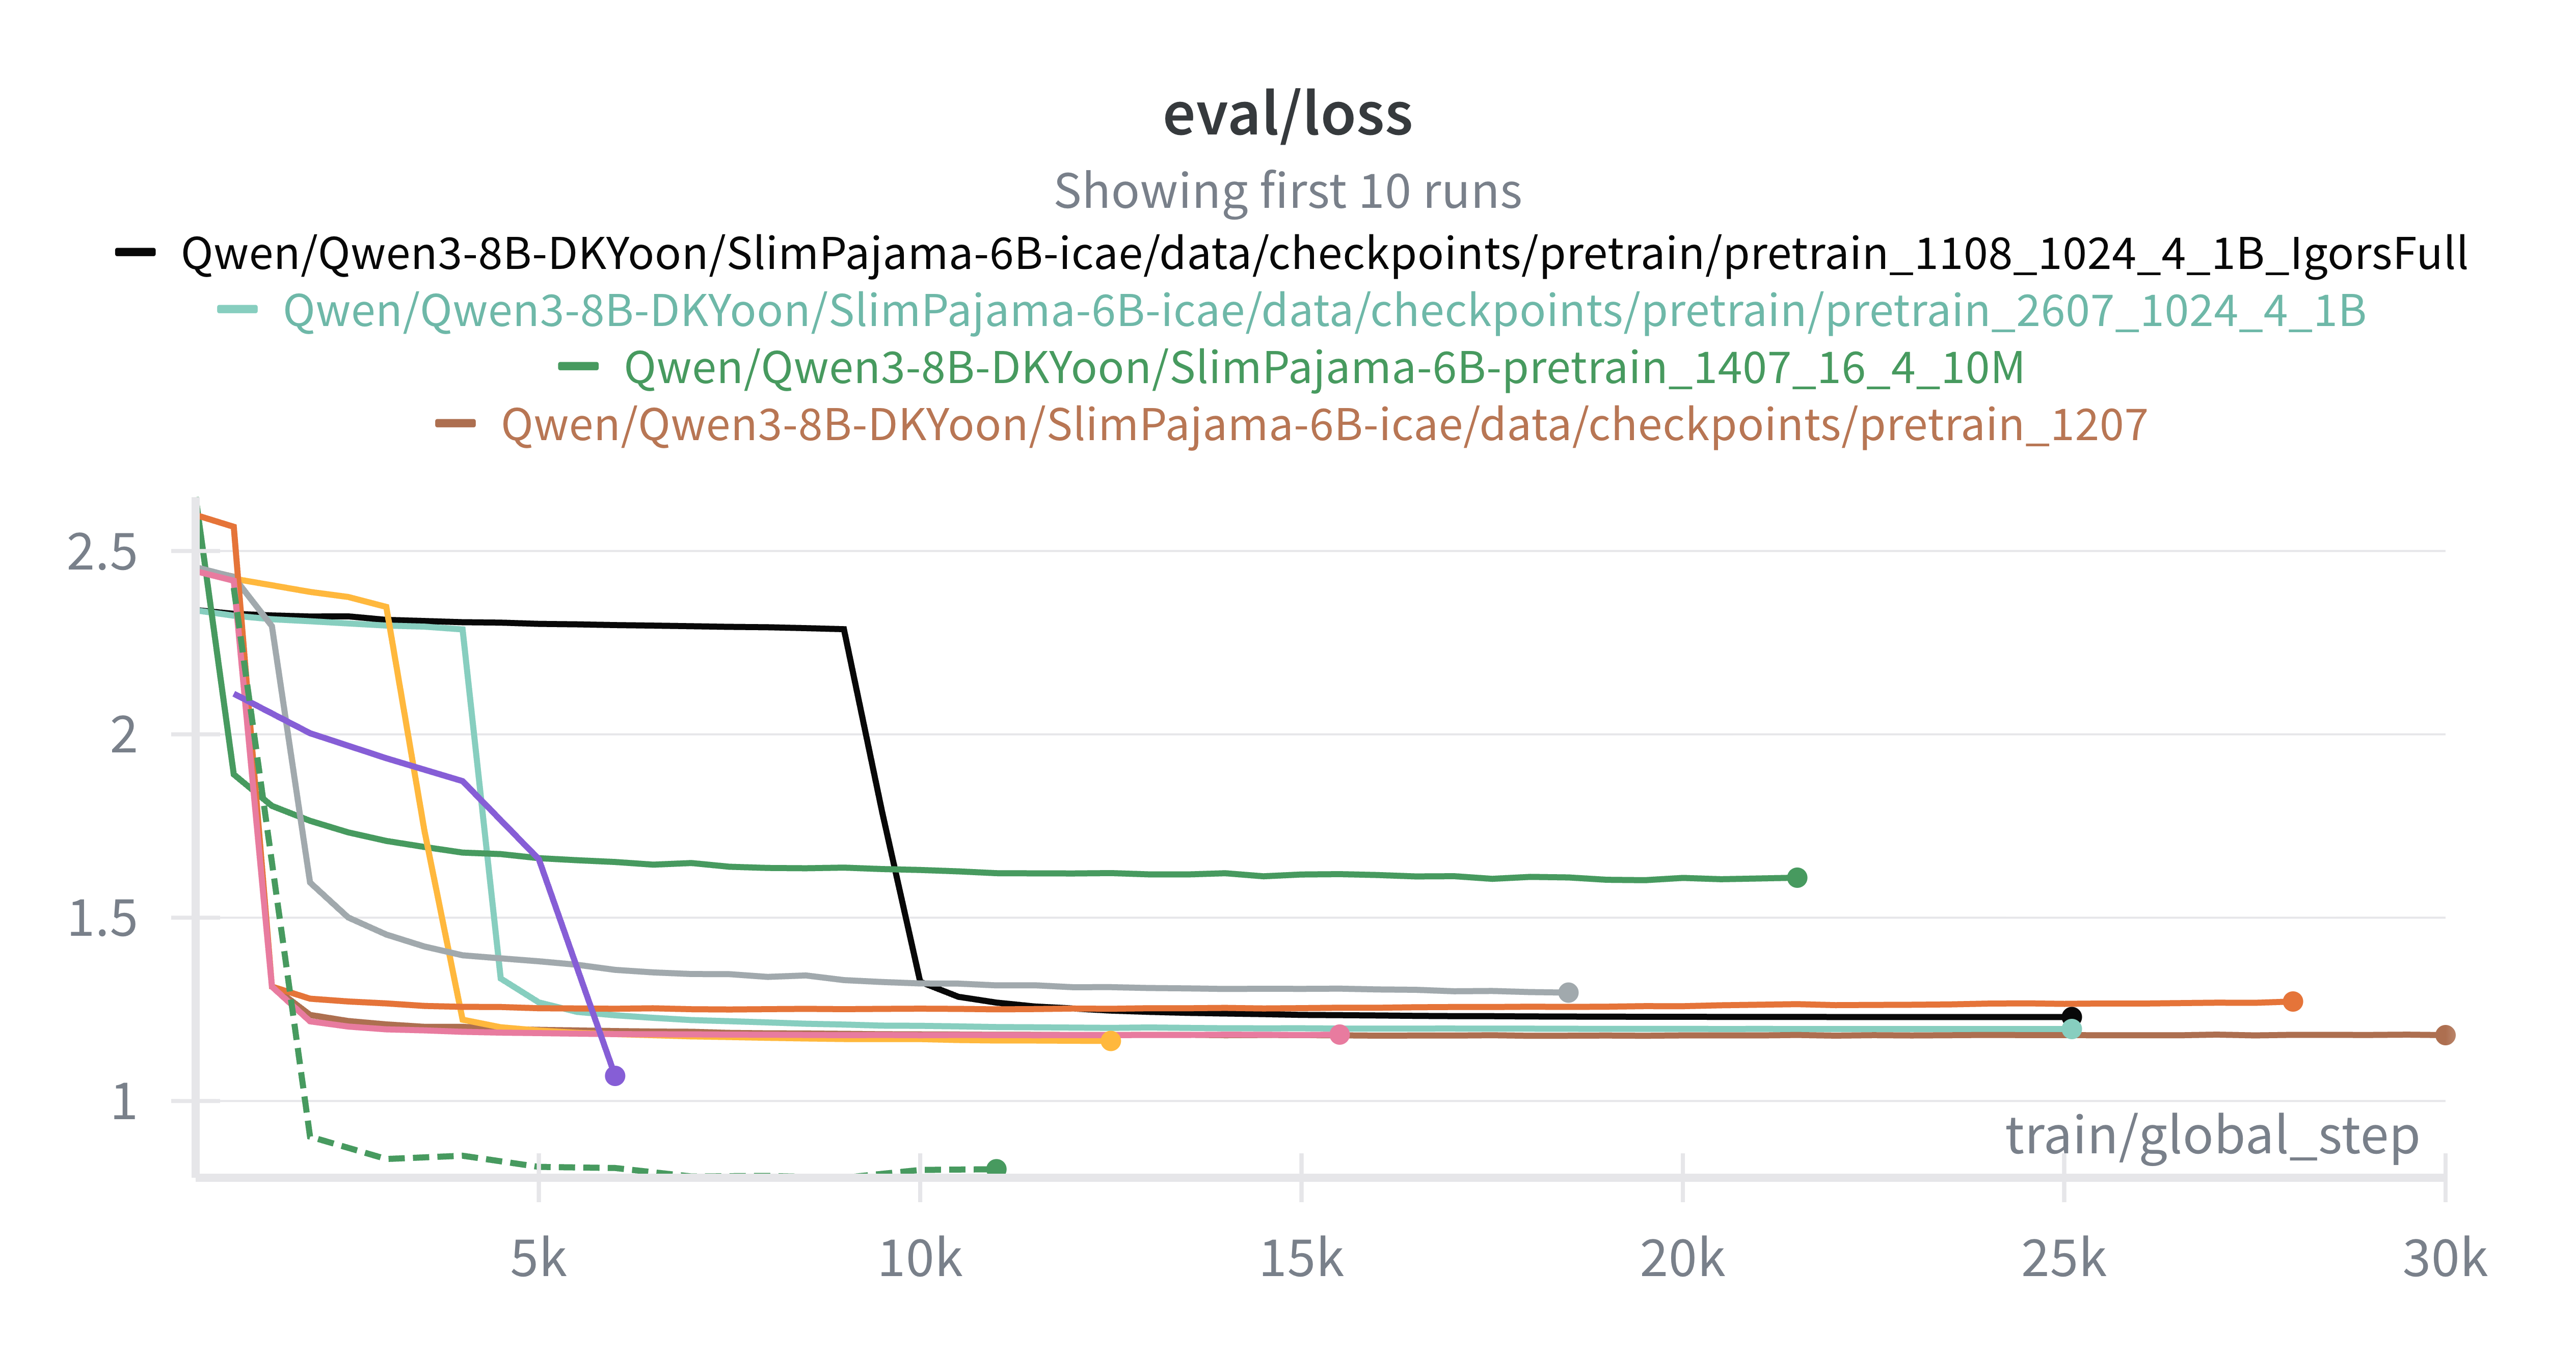
\includegraphics[width=0.9\textwidth]{graphs/ft_losses.png}
  \caption{Fine-tuning loss curves}
  \label{fig:ft_losses}
\end{figure}

\section{Key Metrics}
We report several metrics to evaluate our approach.
As a simple proxy metric, we measure token-wise accuracy —- averaged fraction of the guessed tokens that match the reference trajectory (note: this is measured with teacher forcing).
However, the most important metric is the number of successfully resolved issues on SWE-bench Verified, which directly reflects the model's ability to complete real-world software engineering tasks.
We also measure mean tool-call generation time to assess computational performance.

We note that measuring trajectory length is not particularly meaningful in our setting, as 8B-scale models frequently enter loops where they repeatedly call the same tool, artificially inflating trajectory length without making meaningful progress toward task completion.

% I believe this is not needed? at lease for now
%\subsection{Evaluation}
%In deployment, the accumulated history (trajectory) is first passed to the encoder, which condenses it into memory slots. The decoder (Qwen3) then uses these memory slots, conditioned by the current task prompt, to generate the subsequent action or response. The outcome is that the model operates with a much shorter effective context, improving latency and reducing GPU memory costs during inference.
%The final model is evaluated by deploying it to generate responses iteratively within the ICAE framework on the verified 500 subset of the SWE-bench Verified dataset.



% ========================================
% SECTION 4.5: CODE REPRODUCTION AND TESTING METHODOLOGY
% ========================================
\section{Code Reproduction and Testing Methodology}

\subsection{Code Reproducibility}
We reimplemented the ICAE framework from scratch, as the original authors' code was outdated and difficult to adapt to our experimental needs.
Our implementation is more modular and provides separate training pipelines for both pretraining (PT) and fine-tuning (FT).
We support pretraining on general text datasets (such as SlimPajama) and fine-tuning on both question-answering tasks (SQuAD) and agentic trajectories (SWE-bench).
We provide a link to our code repository\footnote{\url{https://github.com/JetBrains-Research/icae}} for transparency and reproducibility.


